%\documentclass[journal]{IEEEtran}
\documentclass{eplmastersthesis}
%\documentclass{report}
%\usepackage{graphicx}
\usepackage{tikz}
\usetikzlibrary{calc,trees,positioning,arrows,chains,shapes.geometric,%
    decorations.pathreplacing,decorations.pathmorphing,shapes,%
    matrix,shapes.symbols}
\usepackage[siunitx]{circuitikz}
\usepackage[]{tocbibind}
%\usepackage[utf8]{inputenc}
%\usepackage[english]{babel}
%\usepackage[usenames,dvipsnames,svgnames,table]{xcolor}
%\usepackage[style=verbose]{biblatex}
\usepackage[title, titletoc]{appendix}
%\usepackage{refcheck}
%\renewcommand{\includegraphics}[2][]{\fbox{#2}}
\usepackage{wrapfig}
\usepackage{fancyhdr}
%\usepackage[square,sort]{natbib}
%\bibliographystyle{plainnat}

\graphicspath{{./img/}}

\hypersetup{
    colorlinks,
    linkcolor={red!50!black},
    citecolor={red!50!black},
    urlcolor={blue!50!black}
}

\setlength{\headheight}{13.6pt}
\makeatletter
\fancypagestyle{plain}{}
\fancyhf{}
\fancyhead[L]{\textsc{William André}}
\fancyhead[R]{\textsc{\@title, \@subtitle}}
\rfoot{Page \thepage \hspace{1pt} of \pageref{LastPage}}
\fancypagestyle{preamble}{%
    \fancyhf{}
    \fancyhead[L]{\textsc{William André}}
    \fancyhead[R]{\textsc{\@title, \@subtitle}}
    \rfoot{Page \thepage}
}
\fancypagestyle{appendix}{%
    \fancyhf{}
    \fancyhead[L]{\textsc{William André}}
    \fancyhead[R]{\textsc{\@title, \@subtitle}}
    \rfoot{Page \thepage \hspace{1pt} of \pageref{AlmostVeryLastPage}}
}
\fancypagestyle{references}{%
    \fancyhf{}
    \fancyhead[L]{\textsc{William André}}
    \fancyhead[R]{\textsc{\@title, \@subtitle}}
    \rfoot{Page \thepage \hspace{1pt} of \pageref{VeryLastPage}}
}
\makeatother


\makeatletter
\def\@makechapterhead#1{%
  %%%%\vspace*{50\p@}% %%% removed!
  {\parindent \z@ \raggedright \normalfont
    \ifnum \c@secnumdepth >\m@ne
        \huge\bfseries \@chapapp\space \thechapter
        \par\nobreak
        \vskip 10\p@
    \fi
    \interlinepenalty\@M
    \Huge \bfseries #1\par\nobreak
    \vskip 40\p@
  }}
\def\@makeschapterhead#1{%
  %%%%%\vspace*{50\p@}% %%% removed!
  {\parindent \z@ \raggedright
    \normalfont
    \interlinepenalty\@M
    \Huge \bfseries  #1\par\nobreak
    \vskip 40\p@
  }}
\makeatother
 

%\renewcommand{\baselinestretch}{2} % lol xptdr xD

\usepackage{hyperref}
\hypersetup{
    unicode=false,          % non-Latin characters in Acrobat’s bookmarks
    colorlinks=false,       % false: boxed links; true: colored links
    linkcolor=red,          % color of internal links (change box color with linkbordercolor)
    citecolor=green,        % color of links to bibliography
    filecolor=magenta,      % color of file links
    urlcolor=cyan           % color of external links
}

\hyphenation{op-tical net-works semi-conduc-tor}

%\patchcmd{\chapter}{plain}{empty}{}{}
\begin{document}

\pagenumbering{Roman}
% EPL master thesis cover template
%\documentclass{eplmastersthesis}

% Fill in here the information: title, student name, speciality, jury members
\title{EnergyDisaggregation}	% Master thesis title
\subtitle{an open-source EMI based approach}			% Optional subtitle
\author{William \textsc{André}}	% Student name
%\secondauthor{Firstname \textsc{Lastname}}	% Second student name if applicable
\speciality{Computer Science and Engineering}		% Speciality (use one of the following options):
										% Biomedical Engineering
										% Chemical and Materials Engineering
										% Civil Engineering
										% Computer Science
										% Computer Science and Engineering
										% Electrical Engineering
										% Electro-mechanical Engineering
										% Mathematical Engineering
										% Mechanical Engineering
										% Physical Engineering
%\options{Option(s)}		% If required by program commission mention options
\supervisor{Pierre \textsc{Schauss}}	% 1st supervisor name
%\cosupervisor{Firstname \textsc{Lastname}}	% 2nd supervisor name if applicable
\readerone{John \textsc{Aoga}}		% 1st reader name
\readertwo{Siegfried \textsc{Nijssen}}		% 2nd reader name
%\readerthree{Firstname \textsc{Lastname}}	% 3rd reader name
\years{2017-2018}	% Academic year
\maketitle
%\thispagestyle{empty}		% To suppress header and footer on the back of the cover page

\begin{abstract}
The energy disaggregation is an abstract abstraction abstracting the abstract abstrat...
\vspace*{3cm}
\section*{Acknowledgements}
The author would like to thank professor Pierre Schauss for his guidance.
\end{abstract}

%\begin{IEEEkeywords}
%Disaggregation, Energy, NILM
%\end{IEEEkeywords}

\setcounter{tocdepth}{1}
\tableofcontents\thispagestyle{preamble}
\listoffigures\thispagestyle{preamble}
\newpage

\pagenumbering{arabic}
\pagestyle{fancy}

\chapter{Introduction}
\cite{barker2014nilm} %TODO
\section{Defining disaggregation}
The act of disaggregating something is breaking it into multiple parts. In our case, we are looking to break a signal coming from a single, or multiple sources (see \autoref{chapter-improvements}) into different signals coming from different appliances. Once a signal from an appliance is isolated from the global signal, we would also like to know what signal it is and label it.

\subsection{Non Intrusive Load Monitoring}
Actually what we mean by energy disaggregation is Non Intrusive Load Monitoring (often abbreviated NILM). Nonintrusive means that we don't have one sensor per appliance, but rather one sensor per electrical network. The purpose of it is to have a simpler installation, fewer costs and an easier way to update the system.

Load monitoring refers to the electrical load, watching it and try to make suppositions about what it means.

\subsection{Different type of devices}
One thing to keep in mind is that there are a lot of different kind of appliances that use electricity in different kind of ways. Not all appliances need a continuous (meaning the same during all the use-time) AC input at 120V. Actually, there are many types of transformers\cite{harlow2004electric} that don't work the same way and don't necessarily give the same kind of output on a sensor.

There are also appliances that sometimes need a lot of energy, and sometimes don't, like a fridge, an oven or a washing machine. Those appliances often have an identifiable cycle and some studies already address those. But there are also appliances with less predictable cycles, like a drilling machine or other tools.

Waiting for cycles to run in order to identify them could take many minutes, or even hours. This could be a potential problem for some of the applications (see \autoref{section-application})

Having devices using the network in different ways could mean that it would be easy to disaggregate the network, but in practice, it makes it harder because we need multiple ways to collect data, to process them, and eventually make a consensus. This would also mean that the consensus would need to wait for the slowest algorithm to give an output, which would again be a problem for some applications.

Moreover, there are devices that are only in an on/off state and then there are appliances that have multiple states, like a television or a monitor, whose can be on/sleep/off. A laptop or smartphone charger can also have multiple states: on/off but also connected to the laptop or not, and whether the laptop's battery is at full capacity or not.

\section{Current state}
\subsection{Ways to collect data}
A lot of the previous work was focused on slowly acquired data, with the current intensity or more generally the consumed power measured with a sampling rate around 1Hz (like REDD\cite{kolter2011redd}). Others have used a much higher precision to sample the data and even got to a rate of a few GHz\cite{gupta2010electrisense}. This last way to collect data is obviously also much more expensive in hardware: it needs costly measurement tools but it is also harder computationally, needing a faster processor.

Beyond collecting data about the consumption, in order to learn automatically one must also collect data about the state of the appliances. There are various ways to do that. The most used is probably using intrusive sensors, more precisely one sensor per appliance just sensing if that appliance is drawing current from the network or not. In order to eliminate noise, there should be one sensor for every appliance that can send a signal to the nonintrusive sensor.
Some other methods were also designed using thermal imaging\cite{ho2011heatprobe}. This is a bit less intrusive but is also less precise.

There are also multiple public databases if you want to develop an algorithm that needs a lot of data without having to generate it.%http://blog.oliverparson.co.uk/2012/06/public-data-sets-for-nialm.html, http://wiki.nilm.eu/datasets.html




\subsection{Ways to learn}
Like most of the time when building algorithms in artificial intelligence, there are many ways to build a model that will predict the output. All of them have their disadvantages due to the inductive bias and hopefully, most of them have advantages.
\subsubsection{Factorial Hidden Markov Model}
A factorial hidden Markov model (FHMM) is a generalization of the HMM that allows having one HMM per appliance.\cite{parson2014unsupervised} Each appliance can then have multiple hidden states. This solution has been implemented and tested by J. Zico Kolter and Matthew J. Johnson\cite{kolter2011redd} and gave 64.5\% accuracy on the REDD dataset (around 20 monitored appliances).

However, an FHMM needs an exponential number of hidden states: $K^N$ where $K$ is the number of states per appliance and $N$ is the number of appliances. This can become very limiting in real use cases. Some relaxations of the problem exist, like Gibbs sampling, variational Bayes, and variational message passing\cite{parson2014unsupervised}, but this way of solving is still computationally intensive.

\subsubsection{Deep Neural Network}
Deep neural networks are used in a lot of different kinds of applications of machine learning. Some have tried applying this technique to NILM, with satisfying accuracy on some appliances. The authors of \cite{kelly2015neural} decided to use real data from UK-DALE and generated data in a ratio 50:50 for their experiments. Because neural networks can be trained to detect one appliance, they could test the algorithm on only 5 appliances. In order to keep track of the history of what happens in the network, they used a Recurrent Neural Networks and used small batches of offline disaggregation in order to simulate online disaggregation. They also used a neural network (a Denoising AutoeEcoder, DEA) to remove the noise from the read signal. The results are mitigated; some appliances perform really well on the F1 score but some really don't.

Neural Networks are very expensive to build and need several hours of training per appliance on a current high-end GPU.

\subsubsection{Custom designated Algorithm}
custom designated algo\cite{gupta2010electrisense}

\subsubsection{Logical rules}
Sabina Tomkins, Jay Pujara, and Lise Getoor have tried what they call a collective probabilistic approach\cite{tomkins2017disambiguating}. The principle is to group appliances by sets, as some appliances are mostly used together. It should also make it easier to detect as the change on the network is more significant as a set than as a single appliance. Then for each reading and current state, the algorithm outputs a new state. In order to do that, the authors used a hinge loss Markov Random Field (HL-MRF)\cite{bach2015hinge}. This algorithm needs a set of soft logical rules, which are in this case based on the duration of use of the appliances, the different sets of appliances used together, the time and date on which the data is read, and others.

The authors have run their algorithm on the REDD and the DATAPORT datasets, and claim to have reduced errors by previous state-of-the-art algorithms by 50\% and 25\% respectively.

One problem with this algorithm is that it computes what we already know. We need to know when an appliance is likely to be used to detect that it is being used. We need to know which sets of appliances are likely being used together in order to detect one of them. It will probably fail to detect that a light is on during the day, that a heater is on during summer or that air conditioning is on in winter. Although, those are pieces of information that can be very useful when we try to disaggregate a signal, depending on the target (see \autoref{section-target})


\subsection{Other}\label{section-vi}
V-I Trajectory\cite{hassan2014empirical} \cite{lam2007novel}  %https://arxiv.org/pdf/1305.0596.pdf

\cite{do2016applications}%TODO


\section{Applications}\label{section-application}
The purposes of disaggregating such kind of signal are various.

\subsection{Consumption}
The most used is having an estimate of the consumption of each appliance in a household. This means that we don't need to know exactly and immediately when the state of an appliance changes. All we need is that the mean detected uptime of an appliance is close to its true mean uptime. This could help reduce consumption by knowing what appliance is critical. This could also give hints on what appliance could be replaced by a less power consuming one and in how much time the cost can be absorbed by the gain in electricity consumed.

\subsection{Security}
Knowing when an appliance with some risks is plugged and on can also be interesting. Using an iron or a hair straightener for too long could mean that someone forgot to plug it off. Detecting this could be interesting. Also, having an air conditioner running in the winter or a heater running in the summer could be a security issue and need to be reported.

\subsection{Home automation}
Other applications could be used in home automation, to turn on or off something when activity is detected on an appliance for instance.

\section{Target}\label{section-target}
If there are multiple applications, there are also multiple targets. One application can have multiple targets and one target can have multiple applications. A target could be a household, an electricity provider or a factory for instance. A household would have a lot of small appliances, with a few energy-consuming devices, and most of the appliances probably use SMPS (see \autoref{section-smps}). A factory or a workshop probably uses a lot of high energy-consuming tools and machines.

Such differences are to be taken into account when designing an algorithm.


%\section{This thesis path}




\iffalse
Deep neural networks applied to energy disaggregation\cite{kelly2015neural}

REDD: A public data set for energy disaggregation research\cite{kolter2011redd}

NILM redux: The case for emphasizing applications over accuracy\cite{barker2014nilm}

Nonintrusive load monitoring (NILM) performance evaluation\cite{makonin2015nonintrusive}

An in-depth study into using EMI signatures for appliance identification\cite{gulati2014depth}

ElectriSense: single-point sensing using EMI for electrical event detection and classification in the home\cite{gupta2010electrisense}

HeatProbe: a thermal-based power meter for accounting disaggregated electricity usage\cite{ho2011heatprobe}

Applications of Deep Learning Techniques on NILM\cite{do2016applications}

Approaches to Non-Intrusive Load Monitoring (NILM) in the Home\cite{makonin2012approaches}

Non-intrusive load monitoring approaches for disaggregated energy sensing: A survey\cite{zoha2012non}

Disaggregation of
Domestic Smart Meter Energy Data\cite{kelly2016disaggregation}

Algorithms for Energy Disaggregation\cite{fiol2016algorithms}

A survey on metric learning for feature vectors and structured data\cite{bellet2013survey}

\fi\thispagestyle{fancy}
\newpage\chapter{Choice of open-source}
As trying to disaggregate the energy consumption is a problem that has been studied for many years now, many projects already exist. They are mostly commercial projects, and because the technology is evolving but the companies are not always following, those projects fail to grow and persist.

%TODO https://gigaom.com/2011/06/26/5-reasons-google-powermeter-didnt-take-off/
\section{Existing projects}
\subsection{Commercial}
There are a few companies that sell bundles. Amongst the 6 best ones selected by OhmHome\cite{opensourcelist}, only 2 advertise an appliance level detection. One other of the selected ones even only detects appliances that consume above 400W.

Most of the solutions use an easy way to collect necessary data, either by plugging a socket onto the network, or by clamping a sensor around an electricity cable.
\subsection{Open-source}
Few people have tried to make an open source project. The most popular ones are NILMTK\footnote{\url{https://github.com/nilmtk/nilmtk}}\cite{batra2014nilmtk} under Apache 2.0, and NeuralNILM\footnote{\url{https://github.com/JackKelly/neuralnilm}}\cite{kelly2015neural} also under Apache 2.0. Another one is Appliance Energy Detector\footnote{\url{https://github.com/dinoboy197/Appliance-Energy-Detector}}, that is under GNU Affero 3.

None of these projects work directly with sensors. They are all relying on data aquired by others on a long time, mostly using the REDD datasets. This implies that it is working with a power meter, that is in series on the network.
\section{Why GPLv3}
There are quite some researchers working on the NILM problem. A lot of different techniques have been tested and hopefully a lot more will be. While some previous work inspired me in doing this thesis, I hope my work will be used too.

The goal is to have one framework compatible with as much different algorithms as possible. This would greatly improve the comparison between them. Indeed comparing the precision of the algorithms in similar cases is lacking today, yet it is something important.

I am also trying to make the world more transparent and less centralised. A lot of discussions about the IT are centred on the internet being owned by a few companies. Google indeed tried to make a NILM algorithm, and even if it was abandoned\footnote{\url{https://gigaom.com/2011/06/26/5-reasons-google-powermeter-didnt-take-off/}t}, this would have been one more step in one of those companies knowing all about us. Even if it doesn't bother everyone, I am giving the opportunity to the others to make their own system in exchange for their contribution if they can improve it.\thispagestyle{fancy}
\newpage\chapter{Background}
\section{Switch Mode Power Supply}\label{section-smps}
The root of this approach is based on the electromagnetic interference (\acrshort{emi}) induced by switch mode power supplies (\acrshort{smps}). \cite{hesener2010electromagnetic,liu2002high} \acrshort{smps} is a solution proposed by electricians to have more efficient transformers because no current is dissipated as heat by going through resistors. One of its drawbacks is that it induces \acrshort{emi} on the electrical network and therefore to other appliances, possibly disturbing them. Actually, this drawback can be used to our advantage since each device emits a different \acrshort{emi} which could be seen as its signature. This comes from the fact that there are many types of \acrshort{smps}, including buck, boost, buck-boost, boost-buck, zeta, charge pump, flyback, RCC, Forward, push-pull and Ćuk. Of course, there are also many different needs in intensity and power for every appliance which make the signature a step further towards its uniqueness.


As an example one of the \acrshort{smps}, let's take the buck-boost. It is composed of one inductance, one capacitor, one diode, one switch (a transistor), and of course the voltage source and the load. On \autoref{fig:closed_buck-boost} we can see the buck-boost in its closed state. The part in red is the part where current is flowing: the voltage source is loading the inductance, while the capacitor is unloading into the target load. The voltage source can not induce anything in the right part of the schema because of the diode. When the inductance begins to be loaded enough, the voltage change opens the switch.
\begin{figure}[h]
    \centering
    \begin{circuitikz}[scale=2]
    \draw[color=red]
    (0,0) to[voltage source,i^>=$I_s$,v=$V_s$] (0,1)
          to[closing switch] (1,1)
          to[L] (1,0)
          -- (0,0);
    \draw
    (2,1) to[diode] (1,1)
    (2,0) -- (1,0);
    \draw[color=red]
    (2,0) to[C,i^<=$I_c$] (2,1)
          -- (3,1)
          to[generic,label=load,i^<=$I_{load}$,v_<=$V_{load}$] (3,0)
          -- (2,0);
    \end{circuitikz}
    \caption{Closed buck-boost}
    \label{fig:closed_buck-boost}
\end{figure}

We are then in the case shown on \autoref{fig:open_buck-boost}. Again, the part where the current flows is in red. Now, the inductance is unloading into the capacitor and the target load. The capacitor will then be able to be to unload again when the switch will be open.


\begin{figure}[h]
    \centering
    \begin{circuitikz}[scale=2]
    \draw
    (0,0) to[voltage source,i^>=$I_s$,v=$V_s$] (0,1)
          to[opening switch] (1,1)
    (1,0) -- (0,0);
    \draw[color=red]
    (1,1) to[L,i^>=$I_l$] (1,0)
    (2,1) to[diode] (1,1)
    (2,0) -- (1,0);
    \draw[color=red]
    (2,0) to[C,i_>=$I_l$] (2,1)
          -- (3,1)
          to[generic,label=load,i^<=$I_{load}$,v_<=$V_{load}$] (3,0)
          -- (2,0);
    \end{circuitikz}
    \caption{Open buck-boost}
    \label{fig:open_buck-boost}
\end{figure} %TODO sens des fleches ?

The percentage of time that the switch is open is called the duty cycle and controls the potential difference around the load. Because the power of the load may vary, the uptime and downtime are not the same for a fixed duty cycle and source voltage.

Every time the switch is opened or close, there are repercussions on the electrical network.

Also, because of regulations, appliances are equipped with \acrshort{emi} filters. Although they reduce the higher peaks, they also induce smaller variations in the EMI spectrum that make the EMI more unique for every appliance. This is again due to a lot of different filter types and their interactions with the \acrshort{smps}.



\subsection{Electromagnetic Interference}
\acrlong{smps} can induce electromagnetic interferences (\acrshort{emi}) by multiple means. The resistors affect the whole range of frequency, but capacitors and inductances mainly affect the higher frequencies, up to a few GHz.

Because not all the parts of appliances need the same input voltage, there could be multiple \acrshort{smps} inside an appliance. But even with only one \acrshort{smps}, the duty cycle of the converter coupled with the type of converter and the power of the appliance unload very different \acrshort{emi} on the network.


Also, no capacitor is ideal, there are equivalent series resistance (\acrshort{esr}) and inductance (\acrshort{esl}) used to represent it. When current goes through the \acrshort{esr}, there is a voltage drop delayed by the inductance. %TODO is that true? 
This has an effect on the network as well.
\begin{figure}[h]
    \centering
    \begin{circuitikz} \draw
    (0,0) to[R,label=ESR,o-] (2,0) to[L,label=ESL] (4,0) to[C,-o] (6,0);
    \end{circuitikz}
    \caption{Circuit model of non ideal capacitor}
    \label{fig:non_ideal_capacitor}
\end{figure}




\section{Fourier Transform}\label{section:ft}
The Fourier transform (\acrshort{ft}) is a way to represent a function of time into a function of frequencies. It exists for both continuous and discrete functions but as we are reading discrete values, we will focus on the discrete transform.
\begin{equation}S[k] = \sum_{n=0}^{N-1}s[n]e^{\frac{n-2i\pi k}{N}} \qquad \text{for}~0 \leq k < N\end{equation}
Where $N$ is the number of readings of the input signal, the upper case letter ($S$ in this case) is representing the function of frequency, and the lower case letter ($s$ in this case) is representing the function of time.

The inverse is 
\begin{equation} s[k] = \frac{1}{N}\sum_{n=0}{N-1}S[n]e^{\frac{2i\pi kn}{N}}  \qquad \text{for}~0 \leq k < N\end{equation}


When a signal $x[n] = \sum_{k=-\infty}^{+\infty}x[k]\delta[n-k]$ goes through a system $H[h]$, the output $y[n]$ is
\begin{equation}
\begin{array}{rl}
y[n] & = \displaystyle H\{x[n]\}\\
     & = \displaystyle H\{\sum_{k=-\infty}^{+\infty}x[k]\delta[n-k]\} \\
     & = \displaystyle \sum_{k=-\infty}^{+\infty}x[k]H\{\delta[n-k]\} \\
     & = \displaystyle \sum_{k=-\infty}^{+\infty}x[k]h[n-k] \\
\end{array}
\end{equation}
\myequations{Signal through a system}


\subsection{Nyquist-Shannon}\label{section:nyquist}
The Nyquist-Shannon theorem states that in order to not have aliasing in the signal we are processing, the sampling rate must be more than twice the highest frequency of the decomposition of the signal.

This means that if a signal is composed of frequencies higher than the half of the sampling frequency, there will be noise in the signal and the reproduction of a sampled signal would not result in the original signal. As an example, lets take \autoref{fig:nyquist-shannon}. You can see the 3 graphs on the left with 3 different sampling and on the right their respective \acrlong{dft}. The original function is $$f(t) = 1\sin(2\pi60.t) + 0.7\sin(2\pi110.t+5) + 1.2\sin(2\pi256.t)$$. On the first plot, we used a sampling frequency of 800Hz, and on the second and third plot a sampling frequency of 240Hz, the difference between those two that the latter has a shift of 2.0833ms in the sampling. The above sampling has a frequency of more than twice the highest frequency of the function $f(t)$, so there are indeed no problems with the \acrshort{dft}. But the two last sampling have a sampling frequency below the highest frequency so the result of the \acrshort{dft} might not be what we wanted. The amplitude for the 60Hz and the 110Hz components of the wave are correct but there is a component at around 18Hz that wasn't part of the original function.

Note that the inverse \acrshort{dft} don't produce the same function when there is a shifting in the sampling, even though the real part of the \acrshort{dft} is the same, because the imaginary part (not represented) changes the phase of the different component of the function.

The good thing is that the shifting doesn't change the value of the real part of the \acrshort{dft}, in most of the cases, even though the values we get are false.

But in most of the cases means “not all the cases”. On \autoref{fig:nyquist-shannon-2}, the parameters of sampling is the same, but the function has changed. It is now $$f(t) = 1\sin(2\pi60.t) + 0.7\sin(2\pi110.t+5) + 1.2\sin(2\pi300.t)$$. You can see that the higher frequency added up on the readings of 60Hz of the second samling parameters, but did the opposite on the third sampling parameters.


\begin{figure}
    \centering
    \includegraphics[width=\textwidth]{img/nyquist-shannon.png}
    \caption{Example of higher frequencies messing up the DFT}
    \label{fig:nyquist-shannon}
\end{figure}

\begin{figure}
    \centering
    \includegraphics[width=\textwidth]{img/nyquist-shannon-2.png}
    \caption{Another example of higher frequencies messing up the DFT}
    \label{fig:nyquist-shannon-2}
\end{figure}


\subsection{Linear Time Invariant}
Most of the properties described below are true only in linear and time-invariant systems (\acrshort{lti}). If one of those two properties are not satisfied, it is harder or impossible to have a description of the system using Fourier Transforms. Electrical components can be well represented as a \acrshort{lti} system although a perfect \acrshort{lti} system doesn't exist. A resistor or other components' values are a function of the temperature, which is a function of the time. However, using \acrshort{lti} system theory on electrical systems works really good in practice because the variations of the values are expected to be very small.

\subsection{Properties}
The Discrete Fourier Transform (\acrshort{dft}) has a lot of properties but only the ones interesting fir this thesis will be discussed here.
\subsubsection{Linearity}
The response of a system to a sum of multiple signals is the sum of the responses of each individual signal :
\begin{equation}
\begin{array}{rl}
y(t) & = \displaystyle H\{\sum_{i=1}^{N}a_ix_i(t)\} \\
     & = \displaystyle \sum_{i=1}^{N}a_iH\{x_i(t)\} \\
     & = \displaystyle \sum_{i=1}^{N}a_iy_i(t)
\end{array}
\end{equation}
\myequations{Response of a sum of signals}

\subsubsection{Product and convolution}
The convolution of two functions is 
\begin{equation}f(t)*g(t)=\int_{-\infty}^{+\infty}f(\tau)g(t-\tau)d\tau\end{equation}\myequations{Convolution in continuous time}
and in discrete time and frequency :
\begin{equation}f[n]*g[n]=\sum_{k=-\infty}^{+\infty}f[k]g[n-k]\end{equation}\myequations{Convolution in discrete time}

The product in one domain is the convolution in the other domain. In continuous and discrete time respectively, we have
\begin{equation}
    y(t)=x(t)*h(t) \iff Y(j\omega) = X(j\omega)H(j\omega)
\end{equation}

\begin{equation}
    y[n]=x[n]*h[n] \iff Y(e^{j\Omega}) = X(e^{j\Omega})H(e^{j\Omega})
\end{equation}

\subsection{Differentiation}
\begin{equation}
\begin{array}{rl}
x(t)             & = \displaystyle \frac{1}{2\pi}\int_{-\infty}^{+\infty}X(j\omega)e^{j\omega t}d\omega \\
\frac{d}{dt}x(t) & = \displaystyle \frac{1}{2\pi}\int_{-\infty}^{+\infty}X(j\omega)\frac{d}{dt}e^{j\omega t}d\omega \\
                 & = \displaystyle \frac{1}{2\pi}\int_{-\infty}^{+\infty}X(j\omega)j\omega e^{j\omega t}d\omega \\
                 & = j\omega x(t)
\end{array}
\end{equation}

\subsubsection{Shifting}
One interesting property of the \acrshort{ft} is that the result of 

\subsection{Fourier transform in a system}\label{section:fourier-system}
As an example, lets take the simple system described on \autoref{fig:fft_system}\cite{LFSAB1106} :
\begin{figure}
    \centering
    \begin{circuitikz} \draw
    (0,0) to[voltage source,,v=$x(t)$] (0,2) to[R,label=R] (2,2) to[L,label=L] (4,2) to[C,label=C,i=$y(t)$] (4,0) to[] (0,0);
    \end{circuitikz}
    \caption{Simple LRC circuit}
    \label{fig:fft_system}
\end{figure}
Where $x(t)$ is the applied tension and $y(t)$ is the current. We have then
\begin{equation}L\frac{d^2y(t)}{dt^2} + R\frac{dy(t)}{dt}+\frac{1}{C}y(t) = \frac{dx(t)}{dt}\end{equation}\myequations{LRC system input-output relation}
and
\begin{equation}H(j\omega) = \frac{j\omega}{L(j\omega)^2+Rj\omega+\frac{1}{C}}\end{equation}\myequations{LRC system response}

Of course, this is in continuous times and we are measuring on a discrete interval. But this shows that even for a simple system the current flowing 
\thispagestyle{fancy}
\newpage\chapter{Requirements}\label{section:requirements}
The requirements asked to do the thesis were not strictly defined. I had to make choices myself in order to know which directions to take.

One of my main goals was to make energy disaggregation available and affordable for anyone and easily integrable with other projects.

\begin{description}
\item[Hardware] In order for anyone to be able to use the result of the thesis, the hardware should be cheap, or at least not expensive. The range of measurement tools can vary from thousands of euros for a \acrfull{usrp} to a few euro for a split core current transformer.
\item[Code availability] The code should be available so that anyone can tweak it to its own needs. However, it shouldn't need any tweaks for it to run properly \textit{out of the box}. It should also be easy to install the software.
\item[Linking with other projects] Knowing the state of appliances is great, but it is better if we can communicate and share this information with other software.
\item[Computational complexity] The algorithm should not need a dedicated \acrshort{gpu} or some kind of super-computer to run. On the opposite, it should run in the background of a tiny computer without any problem. 
\item[Real time] Most of the time, in order to be usefully linked with other projects, the disaggregation should not wait too long before detecting something.
\item[Appliances] The project is destined to households and the type and number of appliances most of them use. The type of those appliances is mostly electronics and appliances with a switch mode power supply.
\item[Prior] We shouldn't need to know what too much about the habits of the use of the appliances so that something out of the habits has as many chances of being detected as something within the habits.
\end{description}

Another requirement was that it should be open-source, more details on \autoref{section:open-source}.\thispagestyle{fancy}
\newpage\chapter{Implementation}
\section{Hardware}
\begin{wrapfigure}{r}{0.24\textwidth}
    \includegraphics[width=0.9\linewidth]{YHDC-SCT013.jpg}
    \caption{\protect\raggedright YHDC-SCT013}
    %\vspace{-30pt}
    \label{fig:yhdc}
\end{wrapfigure}
As discussed in the introduction, there are multiple ways to collect data. For this project, we wanted a cheap solution easily usable for anyone wanting to use the project; making it more affordable for both users and contributors. This is why we use a generic split-core current transformer, like the one on \autoref{fig:yhdc}. It works using the magnetic field around the wire we monitor to produce a proportional (in this case smaller) current as the one it is clamped around. It is simply wired into the sound card of any computer. This allows getting a sampling of more than 40kHz on most sound cards. However, we are going to sample at only around  4kHz since it seems to be as efficient for our current algorithm.

During the development of the project a laptop was used but since the \acrshort{cpu} usage is very low, a single board computer running Linux (like a Raspberry Pi) should be more than enough to do the job, provided that it has an input on which you can plug the split core current transformer. Note that the split core current transformer can also be plugged into an external USB sound card for instance.


\section{Architecture}
\begin{figure}
    \centering
    \includegraphics[width=\textwidth]{img/diagram.png}
    \caption{Class Diagram}
    \label{fig:class_diagram}
\end{figure}
The project is made to be modular. It is divided into multiple modules aiming at one particular task at a time. The identified tasks are as follow: gather the data, detect when there is a change in the data (i.e. the state of an appliance has changed) and finally detect what appliance it is that has changed. The process is described on \autoref{fig:process_diagram}. Everything is made so that the disaggregation can be made with different types of input data. In this case, we only use a current meter, but the only thing we need to redefine if we change the input data (like adding readings from a voltmeter or/and using the V-I trajectory -- see \autoref{section-vi}) would be to change the distance between two data points.

\tikzset{
    mynode/.style={rectangle,rounded corners,draw=black,very thick, inner sep=0.5em, minimum size=3em, text centered},
    method/.style={ellipse,draw=black,very thick, inner sep=0.01em, minimum size=3em, text centered},
    myarrow/.style={-triangle 45, >=latex', shorten >=1pt, very thick},
    mylabel/.style={text width=7em, text centered} 
} 

\begin{figure}
    \centering
    \begin{tikzpicture}[node distance=2cm, auto]  
    \node[mynode, fill=blue!30] (new_data) {New data};
    \node[mynode, left=1cm of new_data,draw=white] (start) {Start};
    \node[mynode, above right=1cm of new_data] (smoothen_base) {Smoothen Base};
    \node[mynode, below right=1cm of new_data] (smoothen_signal) {Smoothen Signal};
    \node[mynode, below left=of smoothen_signal] (add_data) {Add data to appliance};
    \node[mynode, below right=of smoothen_signal] (new_appliance) {Create new appliance};
    \node[mynode, below = 3cm of smoothen_signal] (signal) {Signal AND New base};
    \node[method, below = 0.5cm of smoothen_signal] (closest) {Get closest};
    \node[method, right = 0.5cm of new_data] (detect) {Detect ?};
    
    \draw[myarrow] (new_data) -- node [text width=2.5cm,below,align=center,sloped] {no} (smoothen_base);
    \draw[myarrow] (new_data) -- node [text width=2.5cm,above,align=center,sloped] {yes} (smoothen_signal);
    \draw[myarrow] (smoothen_signal) -- node [text width=2.5cm,below,align=center,sloped] {Distance below threshold} (add_data);
    \draw[myarrow] (smoothen_signal) -- node [text width=2.5cm,below,align=center,sloped] {Distance above threshold} (new_appliance);
    \draw[myarrow] (add_data) -- (signal);
    \draw[myarrow] (new_appliance) -- (signal);
    \draw[myarrow,dashed] (smoothen_signal) to [out=0,in=50,loop,looseness=4] node [text width=2.5cm,above,align=center,sloped]{Repeat}(smoothen_signal);
    \draw[myarrow] (signal.west) -- ++(-5.6,0) -- ++(0,4) -| (new_data);
    \draw[myarrow] (smoothen_signal.east) -- ++(1.5,0) -- ++(0,5) -| (new_data);
    \draw[myarrow] (smoothen_base.west) -- ++(-1,0) -| (new_data);
    \draw[myarrow] (start) -- (new_data);
    \end{tikzpicture}
    \caption{Process Diagram}
    \label{fig:process_diagram}
\end{figure}


{\color{red}define signal} %TODO

In order to detect when changes in the signal occur, we need to have a base signal. This base signal is the one we should continuously have while there is no change in the network. Because there is a lot of noise due to small variations in the \acrshort{emi} -- due to changes in power needs of the appliances -- , readings errors, and changes in the frequency of the electricity provider -- due to the imbalance of the production and the consumption --, we continuously need to smooth the base signal. This smoothing occurs only if the read signal is not too far from the base signal, which is decided by \texttt{EventDetector}. If it is too far, then the few next readings are taken together and the mean is computed. The difference between this mean and the base signal is expected to be the signal emitted by the new appliance. If that appliance has already been registered, the difference with the mean computed and the base signal should be close to the signal and a copy of the data will automatically be added in the record of the appliance; if not a new appliance will be registered containing the new signal.

To illustrate this, \autoref{fig:state-before} and \autoref{fig:state-after} show the state of the decision algorithm right before and after an event was detected on a dummy example. The red line represents the base signal, that is the agglomeration of all the signals emitted by the appliances emitting \acrshort{emi} at that particular moment. An appliance just changed state, so the current measured signal, which is drawn in blue, has changed. If the difference is big enough, we wait a few moments to try to get rid of the noise in the signal and smooth the difference with the base. That smoothed difference is compared to existing appliances to try to detect which appliance is the cause for changing the signal. The base signal also changes and we get in the state represented on \autoref{fig:state-after}, where the difference between the current signal and the base signal should only be noise.

\begin{figure}
\begin{subfigure}[t]{0.49\textwidth}
    \centering
    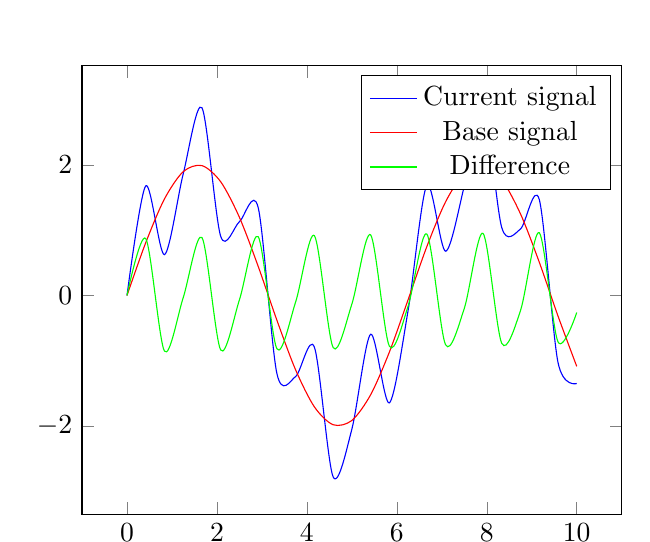
\begin{tikzpicture}[scale=1]
        \begin{axis}[domain=0:10]
            \addplot[mark=none,blue,smooth] {2*sin(deg(x))+sin(deg(5*x))}; 
            \addplot[mark=none,red,smooth] {2*sin(deg(x))};
            \addplot[mark=none,green,smooth] {sin(5*deg(x))};
            \legend{Current signal,Base signal,Difference}
        \end{axis}
    \end{tikzpicture}
    \caption{State right before an event is detected\\}
    \label{fig:state-before}
\end{subfigure}
\begin{subfigure}[t]{0.49\textwidth}
    \centering
    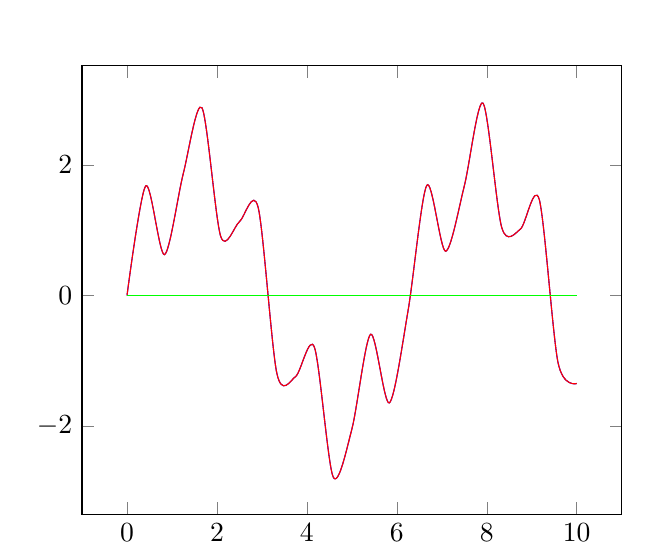
\begin{tikzpicture}[scale=1]
        \begin{axis}[domain=0:10,legend pos=outer north east]
            \addplot[mark=none,blue,smooth] {2*sin(deg(x))+sin(deg(5*x))}; 
            \addplot[mark=none,red,smooth] {2*sin(deg(x))+sin(deg(5*x))};
            \addplot[mark=none,green,smooth] {0};
            %\legend{Current signal,Base signal,Difference}
        \end{axis}
    \end{tikzpicture}
    \caption{State right after an event is detected,\\ and until something else happens on the \\network}
    \label{fig:state-after}
\end{subfigure}
\caption{Change in state}
\label{fig:change-state}
\end{figure}





\section{Algorithms chosen}
\subsection{Fast Fourier Transform}
The raw data we are measuring is actually a waveform. There are some things we can compare between two waveforms, like its maximum values at a certain point, but what we want is the amplitude of every individual frequency outputted by the sum of all appliances. This is done with a \acrshort{ft}.

There are many different types of Fourier Transforms. Because we are sampling the signal, we have to use some kind of \acrshort{dft}. The one chosen is the \acrshort{rfft} because it is optimized to be faster when the input signal is only real.

For reasons enunciated in \autoref{section:nyquist}, we will only look at the real part of the \acrshort{rfft}, as we do not want the results to change because of the difference of phase between the sampling and the input signal.

\subsection{Filtering}
There can be a lot of noise when we measure the current. This has been discussed in \autoref{section-smps}. Also, as we have discussed in \autoref{section:nyquist}, the phase shifting for the sampling may be a problem in some cases.

The combination of those two factors makes the \acrshort{fft} hard to use for comparison between two sets of sampling like we would like to do. In order to illustrate this, \autoref{fig:unfiltered_signal} shows two signals with noise. The first one is the same as the second one but the sampling started 5ms later. 

When we try to filter out the noise by just setting to 0 the values that are below 2 times the mean of \acrshort{fft} values (in this case), we see that the result is not the same depending on the time at which we started sampling. Even though the results of the \acrshort{ft} are indeed different, the sum of absolute value of the differences between the two right graphs is smaller than the one of the two middle graphs.
\begin{figure}
    \centering
    \includegraphics[width=\textwidth]{img/unfiltered.png}
    \caption{Trying to filter out noise}
    \label{fig:unfiltered_signal}
\end{figure}
\begin{figure}
    \centering
    \includegraphics[trim={0 0 0 0.1cm},clip,height=0.99\textwidth, angle =90]{img/filter.png}
    \caption{Filtering out noise with smoothing}
    \label{fig:smooth_signal}
\end{figure}

\subsection{KNN}\label{section:knn}
The \acrshort{knn} algorithm was chosen because it doesn't require training strictly speaking. The training actually is just the gathering of data. This allows seeing quickly how the detecting behaves when the number of data points is growing. However, once the number of training points is bigger, we could easily take another decision technique like a \acrshort{svm}, which is doing much better when the number of training points is huge, and the number of dimensions is big.

There was no need in this case because we were limited by the size of our training set, but \acrshort{knn} also requires to use prototype methods when the number of samples gets bigger. This could be done in a separate thread but needs to be taken into consideration.

Also, in this case, a value of 5 for $k$ was chosen because of the lack of data. But some cross-validation for choosing the value might improve the efficiency of the algorithm.

A problem with this way of using k-NN is however that if there are imprecision's during the sampling of the signal, the \acrshort{dft} could put part of the value of $X[i]$ in $X[i+1]$. For instance, reading a signal of 5kHz as a signal of 5.2kHz. This would lead to a very bad performance of the k-NN.
However, like in \cite{gupta2010electrisense}, we could approximate the \acrshort{dft} by multiple Gaussian curves and use \acrshort{knn} with the parameters of the Gaussian curves.

Another thing worth mentioning is that when I tried to normalize the data around the mean with a variance of 1, the results became really bad. This is because when we normalized the data, we give as much importance to the frequencies that consist mostly of noise than to frequencies that consist mostly of interesting frequencies, as the distance metric we use is simply the euclidian distance between the vector produced by the \acrshort{rfft}.


\subsection{Change in vectors}
In order to detect when there is a change in the \acrshort{dft} values, I used an algorithm inspired by the TCP slow start.

We start by comparing the length (the euclidian norm was chosen) between the base \acrshort{dft} vector and the current reading's \acrshort{dft} vector. If it is below a threshold, we reduce that threshold linearly and repeat that forever. When a reading produces a \acrshort{dft} which difference with a base is greater than the threshold, we augment the threshold exponentially and increment a counter. If the counter gets above a certain value, an event is detected. The counter is decremented every time the difference between the \acrshort{dft} is not greater than the threshold.

The minimum threshold should be close to 0, and the maximum threshold should be big enough to never be a trigger on its own. This way, every event should be detectable. This method ensures that small changes are still detected even if the signal is already strong.

The advantages of this method comparing to the method used by \cite{bruneel2018energy} (the T-Test, see \autoref{section:low-freq}) is that is is much less computationally intensive. However, it needs a tuning of parameters which is less robust than the T-Test, for choosing the rate at which the threshold increases and decreases, as well as choosing how much times the threshold can be exceeded.

In practice, very few false events are detected, and a vast majority of true events are detected. The exception to this is when there are high power appliances that have too much variation over the time. This causes the threshold to be a little too far to detect small appliances.
\thispagestyle{fancy}
\newpage\chapter{Usage}
\section{User Interface}
I developed two user interfaces to interact with the tool. For now, they are complementary and have not the same purpose but they interact in the same way with the core of the tool so making another interface that does all the job can be easily done.
\subsection{CLI}
The \acrlong{cli} developed allows the user to help the algorithm to learn. It will be needed almost exclusively for learning and monitoring of the variables if needed. It prints everything that is happening in the execution of the tool, with a certain level of detail set by the user. You can see the CLI at start time on \autoref{fig:cli-start}. There are also examples of the output produced by the \acrshort{cli} in Appendix \ref{section:cli-dumps}.
\begin{figure}
    \centering
    \includegraphics[width=\textwidth]{img/cli-start.png}
    \caption{The CLI at the start of the soft}
    \label{fig:cli-start}
\end{figure}

There are many things you can do to interact with the software. Here are the current commands :
\begin{description}
\item[\texttt{debug\_level}]This command allows selecting the granularity level of text displayed by the tool. You can choose between \texttt{DEBUG}, \texttt{INFO}, \texttt{WARNING} and \texttt{ERROR}, where \texttt{DEBUG} displays everything that is happening, \texttt{INFO} shows only the useful info needed when the algorithm is already trained, and \texttt{WARNING} and \texttt{ERROR} only show minor and critical error, respectively.
\item[\texttt{delete}] When the algorithm doesn't recognize an appliance, it will not discard the data but create a new appliance with the data associated. This command allows deleting that appliance if it was indeed noise or something unwanted.
\item[\texttt{display}] This is used to launch the GUI if it wasn't started yet or if it was closed.
\item[\texttt{list}] This command list all the appliances known and their current state.
\item[\texttt{load}] You can use \texttt{load} to retrieve the information of an appliance you saved on a previous instance of the program.
\item[\texttt{merge}] You can group two appliances if you think they are similar and that the detection should not make a difference between those appliances.
\item[\texttt{new\_empty\_appliance}] When you try to add a new appliance on a system that already knows some appliances but the new appliance doesn't have a signal that is far enough from a known appliance, chances are that the algorithm will not create a new appliance but associate the new data to the existing appliance. To correct this, you can create a new appliance manually with this command.
\item[\texttt{rename}] Use this to rename an appliance if you don't want generic names like \texttt{item\_0}, \texttt{item\_1},...
\item[\texttt{save}] Once you have trained the algorithm to recognize an appliance, save it with this command in order to be able to recognize it too on other runs of the algorithm.
\item[\texttt{set}] If the algorithm didn't correctly recognize the change of state of an appliance, you may need to set it to its correct state manually with this command.
\item[\texttt{switch}] If the algorithm didn't classify correctly new data, it will assign it to a wrong appliance. You will need to switch it from the wrong appliance to the correct one with this command.
\end{description}

\subsection{GUI}
The \acrlong{gui} doesn't provide any functionality for now but can be very useful to understand what is going on in the algorithm's mind.
\begin{figure}[t]
    \centering
    \includegraphics[width=\textwidth]{img/gui-start.png}
    \caption{The GUI at the start of the soft}
    \label{fig:gui-start}
\end{figure}
An screenshot is shown on \autoref{fig:gui-start}. It was taken a few seconds after the start of the algorithm, so nothing is really learned yet.

The screen is divided into multiple parts :
\begin{itemize}
    \item At the top, there is a representation of the spectrogram of the electrical network. The top of the spectrogram represents the lower frequencies, and the bottom represents the upper frequencies. With the parameters used, the highest frequency we can see is 6kHz. The spectrogram slides with time to the left so that the right of the spectrogram always shows the most recent data. You can see that there are 3 tags on it, labelled \texttt{item\_0} through \texttt{item\_2}. These are the events detected by the algorithm, when it detected them. When an event is detected, the color of the spectrogram changes to give a better visualization.
    \item At the middle of the screen, a representation of the current wave going through the electrical network is represented. There is no interpolation made on the graph so that we see what the algorithm sees.
    \item On the bottom of the screen, there are multiple spectra represented, from left to right :
    \begin{itemize}
        \item The first is the spectrum of the wave currently displayed at the middle of the screen.
        \item The third is the spectrum of the current base. As you will see if you run the program, this will converge to a stable point that is the mean of the few first readings after the base changes.
        \item The second is the absolute value of the difference between the base and the spectrum of the last wave read.
        \item The fourth shows the last spectrum that was classified as being an appliance, i.e. the difference between the mean of the signal read a few times and the base right before changing the base.
        \item The fifth displays the data recorded for the different appliances. There are buttons allowing you to choose which appliance it needs to display.
    \end{itemize}
    All these spectra are made with a real Fourier transform, and only the absolute value of the real part is displayed.
\end{itemize}



\section{Communication with other software}
Because ultimately the main use of the algorithm is not just being able to disaggregate, there is an option allowing to output the states of the appliances on a listening port. We can for instance listen on a port with \texttt{netcat} and send the information with \texttt{python -O Disaggregate.py -p \$PORT -i \$IP}. Every time an event is detected, the appliance and its new state will be outputted on the port.

\section{Training}
In order to have the most accurate data possible, we should train the algorithm one appliance at the time, without anything else making noise. In order to do that, I altered an electrical power strip in order to be able to plug the sensor on it. There should be very few interferences coming from the outside world and indeed, the GUI shows a flat line when nothing is plugged into the power strip.

The training doesn't take a lot of time per appliance, but it needs to be made manually for now. An idea of the general process is the following :
\begin{enumerate}
    \item Plug the new appliance into the power strip.
    \item Change the state of the appliance, let's call it state 1. An event should be detected and the algorithm will create a new appliance and put the data in it.
    \item Change the state of the appliance, let's call it state 2. Again, an event should be detected and a new appliance created.
    \item Switch the data from the last event into a new state of the first appliance.
    \item Set manually the state of the appliance to its real state. Because you manually switched the data, the algorithm doesn't know that the appliance is in state 2 and it won't be able to detect state 1 at the next step. It is indeed not allowed to detect a state it is already in.
    \item Change the state to state 1. Now the algorithm should correctly assign the new data to the correct state of the appliance. If not, switch the data to its correct place and set the state manually.
    \item Change the state to state 2 and do the same as previously if the data is misclassified.
    \item Repeat the last two steps until there are no more errors and the k nearest neighbors are all from the correct state.
\end{enumerate}

However, in some cases, we might need to adapt the manual corrections for some appliances because sometimes an appliance goes through multiple states when you make it go to another state.

\subsection{Different types of appliances}\label{section:appliances}
\subsubsection{Halogen lamp}
\begin{figure}
    \centering
    \includegraphics[trim={0 7cm 0 7cm},clip,width=\textwidth,decodearray={1 0 1 0 1 0}]{img/gui-halogen.png}
    \caption{Representation of the wave of an halogen lamp}
    \label{fig:gui-halogen}
\end{figure}
On \autoref{fig:gui-halogen} you can see the GUI displaying the wave and spectrum emitted by an halogen lamp. Without much surprise, this is very close to a sine wave because an halogen lamp is almost only resistive. However, we can see that the amplitude of the harmonics of 60Hz is not null.

The training of such a device is very easy as there are only two states: on and off.

\subsubsection{Compact Fluorescent Lamp (CFL)}
Now lets take a slightly more complex case : a \acrshort{cfl} lamp. Most of the appliances designed to save energy go through some kind of heating when we start them in order to load the capacitors and the inductor at the desired level.

You can see the wave when we just turned the light on on \autoref{fig:gui-cfl-start}, and when the heating is finished on \autoref{fig:gui-cfl-eco}.
\begin{figure}
\begin{subfigure}{\textwidth}
    \centering
    \includegraphics[trim={0 7cm 0 7cm},clip,width=\textwidth,decodearray={1 0 1 0 1 0}]{img/gui-cfl-start.png}
    \caption{Representation of the wave of a CFL at start}
    \label{fig:gui-cfl-start}
\end{subfigure}
\begin{subfigure}{\textwidth}
    \centering
    \includegraphics[trim={0 7cm 0 7cm},clip,width=\textwidth,decodearray={1 0 1 0 1 0}]{img/gui-cfl-eco.png}
    \caption{Representation of the wave of a CFL after warm up}
    \label{fig:gui-cfl-eco}
\end{subfigure}
\caption{Representation of the waves of the differetn states of a CFL}
\label{fig:gui-cfl}
\end{figure}
They are very similar, the main difference is the phase of the signal captured and the amplitude of the signal. The amplitude of all the frequencies seems to be halved with this particular lamp.

The interesting part in this is that when we turn on the lamp, the algorithm detects the two states above. This lamp will then have 3 states: on, eco, and off.

\subsubsection{Laptop charger}
Now let's take an even more complicated appliance: the laptop charger. The one I tested takes an input AC of 220V and 1.8A, and gives an output DC of 20V and 3.25A.
At first thought, it might seem similar to a CFL, but actually, there is a difference: we can plug it from both ends: one in the laptop and one in the electrical socket. This means there are at least 4 actions for this appliance, with one state per action. Actually, there is a fifth state for the warm-up when we plug it into the laptop.

The different states can be seen on \autoref{fig:gui-laptop-start}, \autoref{fig:gui-laptop-eco} and \autoref{fig:gui-laptop-unplugged}. The states registered for this appliance are : when we plug the charger in the electrical socket without plugging it into the laptop, when we unplug the electrical socket, when we plug it in the laptop when it was already plugged in the electrical socket, and when we unplug it from the laptop but let it plugged into the electrical socket.

There are many things worth noting on those figures. First, we see on \autoref{fig:gui-laptop-eco} that the amplitude of the signal seems limited, probably because the sensor used has reached its limitations. The signal was not amplified, it just came like this through the sensor. By adding more appliances, this becomes obvious. On \autoref{fig:gui-overflow}, you can see that the only thing we can see is a straight top line and a straight bottom line with a quick transition between the two. This was produced using mostly resistive appliances, which should have produced a nice dominant sinewave, and my laptop charger.

Secondly, we can see that the amplitude of the signal is greater on \autoref{fig:gui-laptop-eco} than on \autoref{fig:gui-laptop-start}, which is exactly the opposite of the previous case with the \acrshort{cfl} lamp.

Finally, we see on \autoref{fig:gui-laptop-unplugged} that even if the laptop is not plugged in with the charger, current is still flowing into the charger. This will be the case for other appliances, like a television for instance, which you can shut down without removing the plug but it will still need electricity to be in sleep mode.

\begin{figure}
\begin{subfigure}{\textwidth}
    \centering
    \includegraphics[trim={0 7cm 0 7cm},clip,width=\textwidth,decodearray={1 0 1 0 1 0}]{img/gui-laptop-start.png}
    \caption{Representation of the wave of a laptop charger when just plugged into the laptop and the electrical socket}
    \label{fig:gui-laptop-start}
\end{subfigure}
\begin{subfigure}{\textwidth}
    \centering
    \includegraphics[trim={0 7cm 0 7cm},clip,width=\textwidth,decodearray={1 0 1 0 1 0}]{img/gui-laptop-eco.png}
    \caption{Representation of the wave of a laptop charger after a while when plugged in both laptop and electrical socket}
    \label{fig:gui-laptop-eco}
\end{subfigure}
\begin{subfigure}{\textwidth}
    \centering
    \includegraphics[trim={0 7cm 0 7cm},clip,width=\textwidth,decodearray={1 0 1 0 1 0}]{img/gui-laptop-unplugged.png}
    \caption{Representation of the wave of a laptop charger without plugging it in the laptop}
    \label{fig:gui-laptop-unplugged}
\end{subfigure}
\caption{Representation of the different states of a laptop charger}
\label{fig:gui-laptop}
\end{figure}

\begin{figure}
    \centering
    \includegraphics[trim={0 7cm 0 7cm},clip,width=\textwidth,decodearray={1 0 1 0 1 0}]{img/gui-overflow.png}
    \caption{Representation of the wave with a lot of power}
    \label{fig:gui-overflow}
\end{figure}

\subsubsection{Phone Charger}
The phone charger I tested is taking an input of 220V AC with 0.2A, and outputs a 5V DC 1.2A.
I would have expected to see a similar reaction with the phone charger than with the laptop charger but it wasn't exactly the same. Actually there doesn't seem to be a warm-up phase, and when the charger is not connected to the phone, there is almost no current flowing through it and the difference in amplitude is way too small to be detected, this was predictable though since the current flowing in this charger should be 9 times less than for the laptop charger.

\begin{figure}
    \centering
    \includegraphics[trim={0 7cm 0 7cm},clip,width=\textwidth,decodearray={1 0 1 0 1 0}]{img/gui-phone.png}
    \caption{Representation of the wave of a phone charger}
    \label{fig:gui-phone}
\end{figure}

\thispagestyle{fancy}
\newpage\input{src/Results.tex}\thispagestyle{fancy}
\newpage\chapter{Results and Evaluation}
\section{Results}
\subsubsection{Phase one}
The very first phase in testing the precision of the algorithm was to have a nearly perfect precision on the training phase (i.e., no other appliance is emitting \acrshort{emi}). This is almost trivial because we can just add more points and even if the signal is not always the same, with an increasing number of points, the \acrshort{knn} should choose the right label. Actually, once there was more than $k/2$ examples of the right class (where $k$ is the parameter of the \acrshort{knn}), there were almost never errors while doing the training.
Also, for appliances where there are only 2 status, there are no errors possible because the algorithm can only choose one. This part is more interesting for the laptop charger for instance. The following actions are detected :
\begin{description}
\item[\texttt{charger:plugcharger}] When we plug the charger in the electrical socket without plugging the laptop in
\item[\texttt{charger:unplugcharger}] When we unplug the charger of the electrical socket and the laptop wasn't plugged
\item[\texttt{charger:plug}] When the charger was already in the electrical socket and the laptop is plugged in
\item[\texttt{charger:unplug}] When we unplug the laptop but the charger is still plugged
\item[\texttt{charger:eco}] This should be detected a short while after \texttt{charger:plug}
\end{description}

This works very well in practice. Every one of these individual actions has a high precision. No rigorous methodology was implemented because of the lack of a dataset usable, but I could play with the charger dozens of times without getting any errors. But it worked even better than just recognising those events. For instance, when I first plug the charger into the laptop, 3 events are detected : \texttt{charger:plugcharger}, \texttt{charger:plug} and then \texttt{charger:eco}.

Also, there is only one state that is prevented from being detected : the last one that was detected. So if the last action was \texttt{charger:unplug}, and that I remove the charger from the socket, the 4 other actions have an equal prior probability of being detected. Now the algorithm should make the difference between those actions thanks to the \acrshort{fft}, but since we take the absolute value of it, we could expect that the algorithm has roughly 0.5 chances of picking \texttt{charger:plugcharger} and 0.5 chances of picking \texttt{charger:unplugcharger}. They should after all have the exact opposite effect on the \acrshort{emi} read, so the the absolute value should be the same. But in practice it works really well again.

We discussed in \autoref{section:knn} that 5 might not be the best value for the parameter $k$ of the \acrshort{knn}. In this phase of the training evaluation, $k=1$ would already be a very good decision since all the 5 closest points are generally from the correct class.

\subsubsection{Phase two}
The second phase for evaluation of the algorithm is now to put the data from all the appliances together and see if the algorithm can make the difference between the different appliances, and not only between the different states of an appliance. The only limitation is that we only power up on appliance at the time. The logs have been put in the Appendix \ref{section:cli-dumps}.

Most of the time, there is no problem making differences between different appliances, but sometimes surprising decisions are made. On the log in \autoref{section:a1} for instance, when I plugged my charger inside my laptop, the 5 closest items detected where \texttt{phone-charger:on} instead of \texttt{charger:plug}. Not one of the closest was of the correct class. At least, that was not considered as a correct decision because the points where too far, and a new appliance was created. 

In the log of \autoref{section:a3}, it is even more surprising because there is a detected event right after I plugged my laptop charger when nothing actually happened. It has been assigned to \texttt{halogen:on} with an absolute majority by the \acrshort{knn}, and was accepted because the difference was apparently not too far.

We can see that there are already more difficulties than in the first phase of the evaluation, but the results are not too bad. The only recurrent error, which happened less than 10\% of the time, was a confusion between \texttt{cfl:eco} and \texttt{charger:unplugcharger} after then event \texttt{cfl:on} happened.

\subsubsection{Phase three}
Now, lets do a real test : trying to detect the correct labels when there are other things happening on the network. In order not to have a limitation of the sensor as seen in \autoref{section:appliances} on \autoref{fig:gui-overflow}, I will start by only using appliances that draw little current.

The two appliances I choose are the phone charger and the \acrshort{cfl}. If I first connect the phone charger, almost all the events of the \acrshort{cfl} are correctly classified, without any confusion with any other appliance. The confusion between \texttt{cfl:eco} and \texttt{charger:unplugcharger} mentionned on phase two has a higher probability of happening.

You can see on \autoref{section:a4} some interractions between the appliances when something is wrongly labelled. Because the phone charger was connected, when I shut down the \acrshort{cfl}, an other even was detected. This had a side effect of making the next decision wrong too : because the algorithm thought that the \acrshort{cfl} was still on, the data points corresponding to \texttt{cfl:on} weren't even part of the decision algorithm.

Now, if I do the opposite, the results become worse. When I try to plug/unplug my phone charger when the \acrshort{cfl} is on, the algorithm mostly detects a switch in the state of the \acrshort{cfl}. There is an example of this in \autoref{section:a5}. Surprisingly, one of the times, the points taken into account for the vote of the \acrshort{knn} where all of the correct class \texttt{phone-charger:off} while most of the time only one or less example from the good class are into the 5 closest points.

\section{Evaluation}
\cite{makonin2015nonintrusive}
The lack of rigorous methodology to compute the accuracy of the algorithm makes it hard to compare with previous work. I am however confident that the work produced can be useful and a first step towards a working solution at least as good as proprietary solutions. The limitations we saw on Phase three will most likely be amended with a better split core current transformer.

The information about an appliance are also small and easily downloadable, as it doesn't depend on the home configuration like in \cite{gupta2010electrisense}. If the appliance is not registered yet, you also can train the algorithm really quickly manualy. Letting the algorithm only know the appliances it could possibly know obviously reduces the possibility of false labelling.\thispagestyle{fancy}
\newpage\chapter{Improvements}\label{chapter-improvements}
There are multiple ideas of improvement listed below, which I couldn't implement because of either lack of time, lack of resources, or because it violates the requirements I wanted to keep(\autoref{section:requirements}).
\section{Improve sensor range}
We have seen that there are limitations in the maximum current that we can read with the sensor I used. Using a better sensor would hopefully improve the results of the disaggregation.

\section{Add voltage sensor}
Previous research have shown that adding a sensor able to sample the voltage value can give helpful data to help to disaggregate \cite{bruneel2018energy,hassan2014empirical,lam2007novel}. This can indeed be done without a lot of difficulties with similar hardware as the one used for this thesis. All we would need is a second sound card to do the sampling, and a resistance to reduce the voltage to values that wouldn't harm the sound card.

Because the interesting thing is getting the voltage and the current intensity at exactly the same time, this might however not work really good because the two sound cards are working separately and a difference of a few milliseconds in the synchronisation of the two samplings might be a problem. Also, putting a voltmeter on the electrical panel might require an electrician.

\section{Use multiple sensors}
This might be obvious but instead of using one single sensor for the whole home, we could use one sensor per room for instance. Most electrical panels already split the network into multiple tracks for security reasons. Plugging one sensor per track wouldn't be an issue. 

If we use this, we might also make the difference between fixed appliances (like a ceiling light or a microwave oven) and moving appliances (like a laptop charger). That way, it would be impossible to predict those fixed appliances for something happening in an other room that the one it is in.

It is in some way a compromise between an intrusive and a non-intrusive load monitoring system.

This would work greatly with this system as we have seen that we are having trouble mostly when there are multiple appliances running at the same time, but the detection has a good precision when there is not much other things going on.

\section{Add logical rules}
A model developed prior to this work used mostly logical rules with a \acrshort{hlmrf}. I don't think that using too much logical rules is a good idea but some more than the ones in this can be an improvement. For instance, only allowing the label \texttt{charger:plugcharger} after the label \texttt{charger:unplugcharger} was detected. Reducing the number of labels that can be detected could improve the precision of the algorithm.

However, this could also reduce it. In the same example, if \texttt{charger:unplugcharger} was wrongly detected, I wouldn't be able to detect \texttt{charger:plug} anymore, for instance. 

\section{Not simply add Real Faster Fourier Transforms vectors}
After playing a while with the appliances, I noticed that the vectors do not simply add up when we combine to appliances. This is because the \acrshort{emi} emitted by an appliance depends on the signal it gets in (\autoref{section:fourier-system}).

Even if it depends on the input voltage, and the potential difference should be stable (in an AC way), the input still changes a bit due to the current variations.

\section{Develop automatic learning}
One of the things that is the most problematic in this thesis is the lack of automatic learning.
\subsection{For the metaparameters}
There are multiple metaparameters in the algorithms.
\begin{itemize}
    \item Associator \begin{itemize}
        \item the max distance threshold
        \item $k$ of the \acrshort{knn}
    \end{itemize}
    \item Disaggregate \begin{itemize}
        \item the size of vectors to smoothe the input
        \item the sampling frequency
        \item the sampling size
    \end{itemize}
    \item EventDetector \begin{itemize}
        \item the max distance threshold
        \item the linear decrements of the threshold
        \item the exponential increment of the threshold
    \end{itemize}
\end{itemize}
By running the algorithm with cross-validation of the parameters, we could get better values than the ones I got by manual testing. This would however be time consuming as the algorithm only works on real time. If we wanted to get the best value out of 5 for every one of those parameters by doing a grid search, we would need $5^8=390625$ times the length of the recording. Even if the recording is only 10 minutes long (which would not cover a lot of use cases), this would take more than 7 years to complete on a single computer. This is of course without taking into account that we could launch multiple cross-validations simultaneously on the same computer.

\subsection{For the appliances}
For now, errors made during the training phase have to be corrected manually. This is not practical for automatic learning. A system allowing to make this in an automated way would be a great improvement to the project.

\section{Sample at higher rates}
As done in \cite{gupta2010electrisense}, sampling at a much higher rate might give more insight about the features of certain labels. However, this would also mean that the costs would be greatly increased, going against the requirements of the project.\thispagestyle{fancy}
\newpage\chapter{Conclusion}
Throughout this thesis we have seen that there are multiple approaches to disaggregate the energy consumption. The first methods that have been tried, based only on the instantaneous power consumption readings weren't as promising as the more recent methods using high frequency (range of kHz) and very high frequency (range of MHz) sampling of the current intensity.

The intention of the thesis was to reproduce an algorithm that allowed people to easily set up their own system, by making a solution easy to set up. I wanted also it to be as cheap as possible. I think that both these goals are fulfilled. Actualy all the requirements defined in \autoref{section:requirements} are met. The hardware is easy to get, the code is available\footnote{\url{http://gitlab.com/william.andre/EnergyDisaggregation}} and written in a well known language (Python). It is easy to communicate the information about the disaggregation to an other software, the \acrshort{cpu} usage is low and the response time is less than a few seconds or even faster.

Even though this thesis was greatly inspired by ElectriSense \cite{gupta2010electrisense} and Smappee \cite{bruneel2018energy}, I have searched for improvements. Obviously, the main difference with ElectriSense is that they are using samplings on a much larger frequency band. That larger band allows to have a greater precision, but it also means higher costs which can be an obstacle.\\
The differences with Smappee are both the event detection algorithm and the event association algorithm. While the comparison of those algorithms is difficult because of the lack of automatic learning and automatic testing, the event detection algorithm has at least an advantage regarding its time complexity. This could allow putting more sensors, as suggested in \autoref{chapter-improvements}, because the algorithm running the more often (besides the \acrshort{fft} that is used in both projects) is that event detection; the event association only runs when an event is detected. Also, the method in this thesis can detect multiple different states for one appliance when Smappee only detect on/off states.

However there are still limitations to this technique. These are mainly the lack of an automated learning and the imprecision of the sensor because of it maximum range. I hope and I believe that this will be improved in the future.\thispagestyle{fancy}
\label{LastPage}
\newpage\pagenumbering{Alph}
\pagestyle{appendix}
\renewcommand*{\thepage}{A\arabic{page}}
\begin{appendices}
\chapter{Used appliances}\thispagestyle{appendix}
Some text for the appendix.

\end{appendices}
\label{AlmostVeryLastPage}
\clearpage
\pagenumbering{alph}
\pagestyle{references}
\renewcommand*{\thepage}{B\arabic{page}}

\nocite{*}
\bibliographystyle{IEEEtran}
\bibliography{main}\thispagestyle{references}
\label{VeryLastPage}

\backcoverpage



\iffalse
ACKNOWLEDGEMENTS

TABLE OF CONTENT

TABLE OF FIGURES

I.  INTRODUCTION
	A.  Defining disaggregation
		1)  Different type of devices
	B.  Current state
		1)  Ways to learn
		2)  Ways to collect data
		3)  Other
	C.  Applications

II.  CHOICE OF OPEN-SOURCE
	A.  Existing projects
		1)  Commercial
		2)  Open-source
	B.  Why GPLv3

III.  IMPLEMENTATION
	A.  Architecture
	B.  Algorithms chosen
	C.  Tools
	
IV.  RESULTS

V.  EVALUATION

VI.  IMPROVEMENTS
	A.  Add voltage sensor
	B.  Use multiple sensors
	C.  Develop automatic learning
		1)  For the metaparameters
		2)  For the appliances
	D.  Sample at higher rates

VII.  CONCLUSION

VIII.  REFERENCES

APPENDIX A. USED APPLIANCES
\fi


\end{document}
